\documentclass{article}

\usepackage{microtype}
\usepackage{graphicx}
\usepackage{booktabs}
\usepackage{multirow}
\usepackage{hyperref}
\usepackage{amsmath}
\usepackage{amssymb}
\usepackage{placeins}
\usepackage{tikz}
\usetikzlibrary{shapes.geometric, arrows.meta, positioning}
\usepackage{algorithm}

\usepackage{icml2026}

\usepackage[capitalize,noabbrev]{cleveref}

\icmltitlerunning{Credit Risk Scoring from Mobile Money Behavioral Features}

\begin{document}

\twocolumn[
  \icmltitle{Credit Risk Scoring from Mobile Money Behavioral Features:\\
    A Large-Scale Study on Real Ghanaian Transaction Data}

  \begin{icmlauthorlist}
    \icmlauthor{Anonymous}{anon}
  \end{icmlauthorlist}

  \icmlaffiliation{anon}{Anonymous Institution}
  \icmlcorrespondingauthor{Anonymous}{anonymous@anonymous.com}
  \icmlkeywords{credit scoring, mobile money, financial inclusion, Ghana, machine learning, temporal feature engineering}

  \vskip 0.3in
]

\printAffiliationsAndNotice{}

\begin{abstract}
Mobile money (MoMo) platforms serve as the primary financial
infrastructure for millions of unbanked people in sub-Saharan Africa,
yet credit risk assessment remains hampered by the absence of
traditional credit bureau data.
We present a large-scale empirical study using 374 million real
transactions from 222,618 borrowers on a Ghanaian MoMo platform,
applying a temporal feature engineering framework that derives 47
behavioral features exclusively from pre-loan transaction history.
We identify and correct a critical data leakage pattern,the
\emph{index-loan temporal cutoff},and show it inflates AUC-ROC to
1.0 without correction.
After full correction, gradient boosting models achieve AUC-ROC of
0.732 for strict default prediction without any credit bureau features.
We further find that a calibrated synthetic benchmark
overestimates real-world discriminative performance by approximately
15 percentage points, suggesting that synthetic pre-training should be
treated as an optimistic upper bound.
\end{abstract}

\section{Introduction}

Sub-Saharan Africa has experienced explosive growth in mobile money
adoption, with Ghana ranking among the continent's most active markets:
over 65 million registered MoMo accounts and GHS 278 billion in
transaction value as of 2023~\cite{ghana2024mobile}.
For tens of millions of individuals, mobile money is their \emph{only}
financial footprint,the sole structured record of income, spending,
and financial behavior.
Yet credit scoring in this context remains largely unsolved: traditional
bureaus are absent or nascent, and most micro-lenders rely on simple
heuristics or relationship-based lending.

Recent work has demonstrated that behavioral traces from digital
platforms can predict creditworthiness even without conventional credit
history~\cite{bjorkegren2020behavior,francis2019effective}.
However, most published studies use small proprietary samples, synthetic
proxies, or data from markets with stronger baseline infrastructure.
The unique characteristics of West African MoMo ecosystems,dense
transaction graphs, high loan turnover, and informal economic patterns —
are largely unstudied at scale.

We address this gap with a large-scale study on real transaction data
from a Ghanaian MoMo provider.
Our contributions are:
\begin{enumerate}
  \item \textbf{Scale:} The largest published credit scoring study on
        real African MoMo data: 374M transactions, 222K borrowers.
  \item \textbf{Temporal leakage formalization:} We identify and correct
        a systematic leakage pattern,the index-loan temporal cutoff —
        and show it inflates AUC to 1.0.
  \item \textbf{Real-data baseline:} AUC-ROC of 0.732 for strict default
        prediction using behavioral features alone.
  \item \textbf{Synthetic-to-real gap:} We compare results to a prior
        synthetic benchmark~\cite{anonymous2026seqcredit}, finding that
        synthetic calibration \emph{overestimates} real-world
        performance by $\approx$15 percentage points.
\end{enumerate}

\section{Related Work}

Credit scoring from alternative data has attracted growing attention in
emerging markets~\cite{bjorkegren2020behavior,francis2019effective,ngwenya2024credit}.
\citet{bjorkegren2020behavior} show smartphone behavioral signatures
predict repayment in developing markets; \citet{ngwenya2024credit} apply
logistic regression to alternative data in Africa.
Gradient boosting models,XGBoost~\cite{chen2016xgboost} and
LightGBM~\cite{ke2017lightgbm},consistently dominate tabular credit
benchmarks, a pattern we confirm on real MoMo data.
Mobile money as a financial inclusion vehicle specific to sub-Saharan
Africa is surveyed by \citet{osabutey2024mobile} and documented
institutionally by \citet{africanenda2025siips}.
To our knowledge, no prior work evaluates behavioral credit scoring at
this scale on real West African MoMo data with explicit temporal leakage
controls.

\section{Data}

\subsection{Dataset}

Our data is drawn from a proprietary transaction log of a major Ghanaian
MoMo provider covering December 2025 to February 2026,approximately
90 days of activity.
All identifiers are hashed and anonymized.
The raw table contains 374,295,424 rows across 12 columns:
transaction timestamp, transaction type (243 distinct values), debit
and credit party IDs, account types, and transaction amount in GHS.
We identify 474,312 unique borrowers as customers who received at least
one loan disbursement (``Loan Payment Via API'') from the platform
lender (\texttt{LENDER\_ID = E7C89F8C4A27F173}).

\subsection{Temporal Cutoff and Label Design}

A naive pipeline computing features over the full observation window
allows post-loan repayment signals to directly encode the label —
inflating AUC-ROC to $\approx$1.0.
We prevent this with the \emph{index-loan cutoff}: for each borrower,
features are derived exclusively from transactions occurring
\emph{strictly before} their most recent loan disbursement; labels are
derived from events \emph{strictly after} it.

To address right-censoring,borrowers whose index loan occurred near
the end of the window have insufficient followup time,we apply a
30-day minimum followup filter, retaining 223,081 borrowers.
Of these, 222,618 have at least one pre-loan transaction and thus
non-empty feature vectors; 463 are dropped at merge.
We define two prediction targets:
\begin{itemize}
  \item $y_{\text{default}}$: 1 if the borrower made \emph{zero}
        principal or interest repayments after their index loan.
  \item $y_{\text{bad}}$: 1 if the borrower defaulted \emph{or}
        incurred a penalty after their index loan.
\end{itemize}

Label distributions are shown in Table~\ref{tab:labels}.

\begin{table}[h]
\caption{Label distribution after 30-day followup filter ($n=223{,}081$).
  The 4.4\% strict default rate reflects borrowers with \emph{zero}
  repayments in the observation window.}
\label{tab:labels}
\vskip 0.1in
\begin{center}
\begin{small}
\begin{tabular}{lrr}
\toprule
Label & Count & \% \\
\midrule
Good (repaid, no penalty)   & 93,272  & 41.8\% \\
Risky (repaid with penalty) & 120,074 & 53.8\% \\
Default (never repaid)      & 9,735   &  4.4\% \\
\midrule
$y_{\text{default}}$ positive rate & 9,735   &  4.4\% \\
$y_{\text{bad}}$ positive rate     & 129,809 & 58.2\% \\
\bottomrule
\end{tabular}
\end{small}
\end{center}
\vskip -0.1in
\end{table}

\section{Feature Engineering}

We extract 47 user-level aggregate features from the pre-cutoff
transaction window, grouped into eight semantic categories:
(1)~volume and amount statistics (total, mean, std, CV, min/max/median);
(2)~transaction type mix across 9 semantic categories (transfer,
cash-out, payment, airtime/data, betting, FSI interop, loan repayment
principal/interest, loan penalty);
(3)~temporal patterns (cyclical hour-of-day and day-of-week encodings,
night/early-morning/weekend fractions);
(4)~loan history on \emph{prior} loans only (count, volume,
disbursements, repayments, penalties);
(5)~repayment behavior (repayment ratio, total principal and interest
repaid relative to loan volume);
(6)~inflow dynamics (total inflow, average inflow, cash-in deposits);
(7)~behavioral diversity (unique recipients, unique transaction types,
recipient concentration);
(8)~derived cash-flow features (net flow, inflow-outflow ratio,
transactions per day, average inter-transaction gap).

The 243 raw transaction type strings are mapped to 9 semantic categories
via rule-based pattern matching.
The full feature list is in Appendix~\ref{app:features}.

\section{Experiments}

\subsection{Setup}

We evaluate four classifiers: Logistic Regression (LR), Random
Forest (RF), XGBoost~\cite{chen2016xgboost}, and
LightGBM~\cite{ke2017lightgbm}.
All models are evaluated via 5-fold stratified cross-validation
(seed~=~42) on 222,618 borrowers.
Features are standardized with a \texttt{StandardScaler} fit on each
training fold.
We report mean AUC-ROC, AUC-PR, F1, Brier score, and Expected
Calibration Error (ECE) across folds.
Statistical significance between model pairs is assessed with 1,000
bootstrap iterations at $p < 0.05$.
Hyperparameters are listed in Appendix~\ref{app:hyperparams}.

\subsection{Results}

Table~\ref{tab:results} reports results for both targets.
For $y_{\text{default}}$, XGBoost achieves the best AUC-ROC
($0.732_{\pm.010}$), with all gradient boosting models clustered in
$0.723$--$0.732$ and LR trailing at $0.709_{\pm.010}$.
For $y_{\text{bad}}$, the task is better-conditioned (58.2\% positive
rate): LightGBM leads at AUC-ROC $0.729_{\pm.002}$ with excellent
calibration (ECE 0.067), while XGBoost achieves the best F1 (0.741)
but with poor calibration (ECE 0.363).
ROC curves are shown in Figure~\ref{fig:roc}.

\begin{table*}[tp]
\caption{5-fold CV results on 222,618 borrowers (30-day followup
  filter). Means across folds; subscript shows per-fold std.
  $y_{\text{default}}$: strict default (zero repayments).
  $y_{\text{bad}}$: default or penalised.}
\label{tab:results}
\vskip 0.1in
\begin{center}
\begin{small}
\begin{tabular}{llccccc}
\toprule
Target & Model & AUC-ROC & AUC-PR & F1 & Brier & ECE \\
\midrule
\multirow{4}{*}{$y_{\text{default}}$}
  & XGBoost             & $\mathbf{0.7317}_{\pm.010}$ & \textbf{0.1120} & 0.1566 & 0.1749 & 0.3175 \\
  & LightGBM            & $0.7289_{\pm.008}$ & 0.1105 & 0.1570 & 0.1748 & 0.3187 \\
  & Random Forest       & $0.7229_{\pm.008}$ & 0.1007 & \textbf{0.1611} & \textbf{0.1620} & \textbf{0.3168} \\
  & Logistic Regression & $0.7093_{\pm.010}$ & 0.0971 & 0.1394 & 0.2194 & 0.3966 \\
\midrule
\multirow{4}{*}{$y_{\text{bad}}$}
  & LightGBM            & $\mathbf{0.7293}_{\pm.002}$ & \textbf{0.7791} & 0.6988 & \textbf{0.2095} & \textbf{0.0666} \\
  & XGBoost             & $0.7274_{\pm.003}$ & 0.7774 & \textbf{0.7407} & 0.3596 & 0.3634 \\
  & Random Forest       & $0.7185_{\pm.003}$ & 0.7684 & 0.6886 & 0.2149 & 0.0735 \\
  & Logistic Regression & $0.6907_{\pm.004}$ & 0.7467 & 0.6660 & 0.2228 & 0.0735 \\
\bottomrule
\end{tabular}
\end{small}
\end{center}
\vskip -0.1in
\end{table*}

\subsection{Discussion}

\textbf{Leakage impact.}
Without the index-loan cutoff, AUC-ROC reaches 1.0,a trivial
outcome driven by post-loan repayment features encoding the label.
After correction, AUC-ROC is 0.732: a meaningful but honest result.

\textbf{Severe class imbalance shapes metrics.}
The 4.4\% default rate makes AUC-PR and F1 low by construction for
$y_{\text{default}}$ (AUC-PR $\approx$ 0.11, F1 $\approx$ 0.16),
even though AUC-ROC of 0.732 represents genuine discrimination.
Practitioners deploying these models should rely on probability scores
with proper recalibration rather than fixed-threshold F1.

\textbf{Synthetic-to-real gap.}
A companion study~\cite{anonymous2026seqcredit} evaluated the same
feature framework on a calibrated 10,000-user synthetic MoMo dataset,
reporting XGBoost AUC-ROC of 0.881 and LightGBM 0.878.
On real data the same models achieve 0.732 and 0.729,a gap of
approximately 15 percentage points, driven by informal economy noise,
irregular income cycles, and user-level data sparsity absent from
synthetic calibration.

\textbf{Feature engineering dominates model choice.}
No pairwise comparison reaches statistical significance at 5\% for
either target, despite $n = 222$K.
This convergence suggests the performance ceiling is set by the feature
representation, not the model family,consistent with prior work in
tabular ML~\cite{ngwenya2024credit}.

\textbf{Calibration varies by task.}
For $y_{\text{bad}}$ (balanced classes), LightGBM delivers both strong
discrimination and excellent calibration (ECE 0.067), making its
probability scores directly actionable for loan pricing.
For $y_{\text{default}}$ (4.4\% positive), all models show high ECE
(0.32--0.40), requiring post-hoc recalibration before deployment.

\begin{figure}[htbp]
\centering
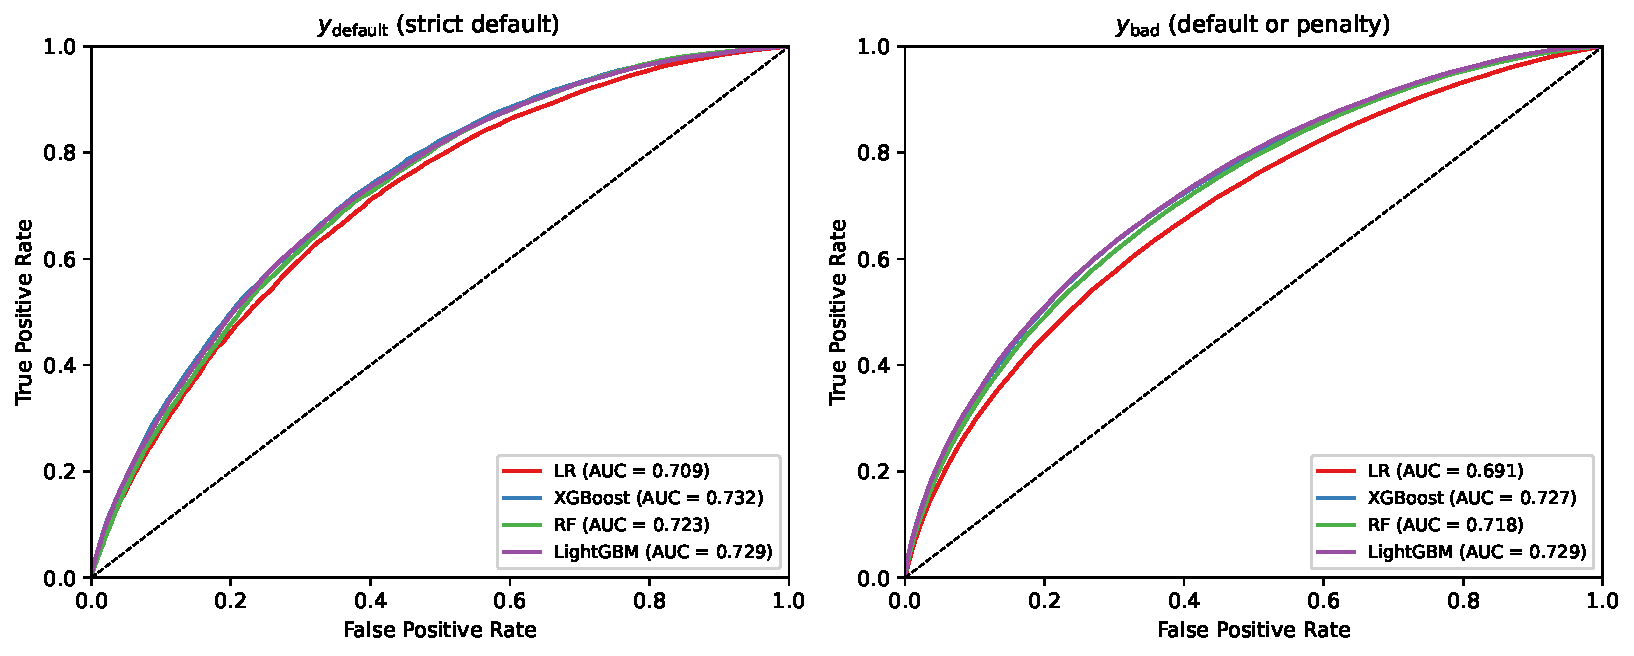
\includegraphics[width=\columnwidth]{roc_curves}
\caption{Out-of-fold ROC curves for all four classifiers on both
  prediction targets ($n=222{,}618$, 5-fold OOF).
  AUC values match Table~\ref{tab:results}.}
\label{fig:roc}
\end{figure}

\section{Conclusion}

We present a large-scale credit scoring study on real West African
mobile money data, demonstrating that behavioral features derived from
transaction history predict strict default with AUC-ROC of 0.732 on
222,618 Ghanaian borrowers,without any credit bureau features.
We formalize the index-loan temporal cutoff as a necessary leakage
control, and establish that a calibrated synthetic benchmark
overestimates real-world performance by $\approx$15 percentage points.
Future work will extend the pipeline with transaction-level LSTM models
to assess whether temporal order carries additional signal beyond
aggregate summaries, and will explore fairness and interpretability
requirements for deployment.

\section*{Impact Statement}

This work advances credit access for unbanked populations in sub-Saharan
Africa by demonstrating the viability of behavioral credit scoring from
mobile money data.
Potential risks include automated credit denial for vulnerable groups;
all user identifiers are hashed and anonymized.
Models evaluated here require interpretability and fairness audits before
any deployment; responsible deployment should include demographic impact
assessments and mechanisms for human review.

\bibliography{references}
\bibliographystyle{icml2026}

\clearpage
\onecolumn
\appendix

\section{Pipeline Pseudocode}
\label{app:pseudocode}

Algorithm~\ref{alg:cutoff} formalizes the index-loan temporal cutoff
and right-censoring filter that are the core methodological
contributions of this work.

\begin{algorithm}[h]
\caption{Index-loan cutoff and right-censoring filter}
\label{alg:cutoff}
\begin{algorithmic}
\REQUIRE Transaction log $\mathcal{T}$, min followup $d = 30$ days
\ENSURE Feature matrix $X$, label vector $y$
\STATE $t_{\max} \gets \max_{r \in \mathcal{T}} r.\mathit{ts}$
\STATE $t_{\text{cutoff}} \gets t_{\max} - d$
\FOR{each borrower $u$}
  \STATE $t^*_u \gets \max\{r.\mathit{ts} : r \in \mathcal{T}_u,\ r.\mathit{type} = \textsc{LoanDisb}\}$
  \IF{$t^*_u > t_{\text{cutoff}}$}
    \STATE \textbf{drop} $u$ \COMMENT{insufficient followup}
  \ELSE
    \STATE $\mathcal{T}^-_u \gets \{r \in \mathcal{T}_u : r.\mathit{ts} < t^*_u\}$ \COMMENT{pre-loan}
    \STATE $\mathcal{T}^+_u \gets \{r \in \mathcal{T}_u : r.\mathit{ts} > t^*_u\}$ \COMMENT{post-loan}
    \STATE $X_u \gets \textsc{ExtractFeatures}(\mathcal{T}^-_u)$
    \STATE $y_u \gets \mathbf{1}[\text{no repayments in } \mathcal{T}^+_u]$
  \ENDIF
\ENDFOR
\end{algorithmic}
\end{algorithm}

\section{Feature Engineering Pipeline}
\label{app:flowchart}

\begin{figure}[h]
\centering
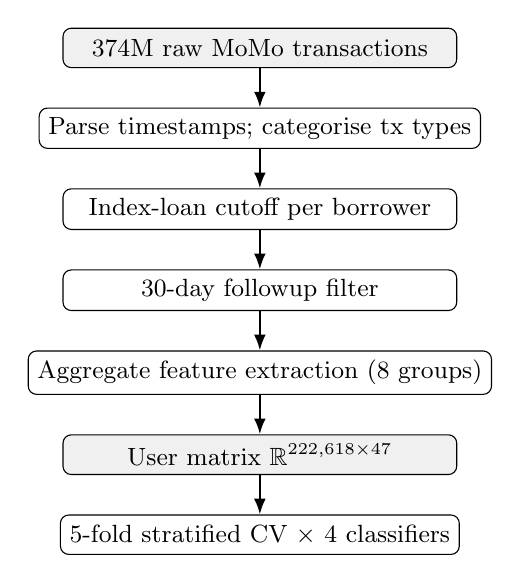
\begin{tikzpicture}[
  node distance=0.5cm,
  box/.style={rectangle, draw, rounded corners=3pt, text centered,
              minimum width=5.0cm, minimum height=0.5cm,
              font=\small, fill=white},
  hibox/.style={rectangle, draw, rounded corners=3pt, text centered,
              minimum width=5.0cm, minimum height=0.5cm,
              font=\small, fill=gray!12},
  arr/.style={-{Latex[length=2mm]}, thick}
]
\node[hibox] (raw)  {374M raw MoMo transactions};
\node[box, below=of raw]  (parse) {Parse timestamps; categorise tx types};
\node[box, below=of parse] (cut)  {Index-loan cutoff per borrower};
\node[box, below=of cut]  (filt) {30-day followup filter};
\node[box, below=of filt] (feat) {Aggregate feature extraction (8 groups)};
\node[hibox, below=of feat] (mat)  {User matrix $\mathbb{R}^{222{,}618 \times 47}$};
\node[box, below=of mat]  (cv)   {5-fold stratified CV $\times$ 4 classifiers};

\draw[arr] (raw)   -- (parse);
\draw[arr] (parse) -- (cut);
\draw[arr] (cut)   -- (filt);
\draw[arr] (filt)  -- (feat);
\draw[arr] (feat)  -- (mat);
\draw[arr] (mat)   -- (cv);
\end{tikzpicture}
\caption{End-to-end pipeline from raw transactions to cross-validated
  model evaluation.}
\label{fig:pipeline}
\end{figure}

\section{Full Feature List}
\label{app:features}

Table~\ref{tab:features} lists all 47 features.
Four balance-at-loan features (\dag) are not available from the raw
transaction log and are set to zero; they are retained for interface
compatibility with the synthetic benchmark~\cite{anonymous2026seqcredit}.

\begin{table*}[h]
\caption{All 47 user-level features by category.}
\label{tab:features}
\vskip 0.05in
\begin{center}
\begin{scriptsize}
\begin{tabular}{p{2.0cm}p{12.0cm}}
\toprule
Category & Features \\
\midrule
Volume \& amount
  & \texttt{obs\_txn\_count}, \texttt{total\_volume},
    \texttt{avg\_transaction\_amount}, \texttt{median\_transaction\_amount},
    \texttt{std\_transaction\_amount}, \texttt{max\_transaction\_amount},
    \texttt{min\_transaction\_amount}, \texttt{cv\_transaction\_amount} \\
\addlinespace
Tx type mix
  & \texttt{pct\_transfers}, \texttt{pct\_cashouts},
    \texttt{pct\_payments}, \texttt{pct\_airtime},
    \texttt{pct\_betting}, \texttt{pct\_fsi} \\
\addlinespace
Temporal
  & \texttt{pct\_night\_txns},
    \texttt{pct\_early\_morning\_txns},
    \texttt{pct\_weekend\_txns} \\
\addlinespace
Loan history
  & \texttt{n\_loans\_received}, \texttt{total\_loan\_volume},
    \texttt{avg\_loan\_amount}, \texttt{max\_loan\_amount} \\
\addlinespace
Repayment
  & \texttt{n\_principal\_repayments}, \texttt{n\_interest\_repayments},
    \texttt{n\_penalty\_txns}, \texttt{total\_principal\_repaid},
    \texttt{total\_interest\_repaid}, \texttt{total\_penalties\_paid},
    \texttt{total\_repaid}, \texttt{loan\_repayment\_ratio} \\
\addlinespace
Inflow
  & \texttt{total\_inflow}, \texttt{avg\_inflow\_amount},
    \texttt{total\_cash\_in} \\
\addlinespace
Diversity
  & \texttt{unique\_recipients}, \texttt{unique\_txn\_types},
    \texttt{unique\_senders}, \texttt{recipient\_concentration} \\
\addlinespace
Cash-flow
  & \texttt{net\_flow}, \texttt{inflow\_outflow\_ratio},
    \texttt{account\_age\_days}, \texttt{transactions\_per\_day},
    \texttt{avg\_hours\_between\_txns}, \texttt{loan\_to\_total\_volume\_ratio},
    \texttt{pct\_credit\_transactions},
    \texttt{loan\_timing\_in\_sequence}$^\dag$,
    \texttt{avg\_balance\_at\_loan}$^\dag$,
    \texttt{min\_balance\_at\_loan}$^\dag$,
    \texttt{balance\_to\_loan\_ratio\_at\_disbursement}$^\dag$ \\
\bottomrule
\end{tabular}
\end{scriptsize}
\end{center}
\vskip -0.1in
\end{table*}

\section{Model Hyperparameters and Infrastructure}
\label{app:hyperparams}

All models use 5-fold stratified cross-validation (seed~42) with
\texttt{StandardScaler} fit on each training fold.
Experiments ran on Azure Databricks (serverless runtime, Apache Spark
3.x); feature engineering processed 374M rows in a single distributed
pass via PySpark aggregations.

\begin{table}[h]
\caption{Hyperparameters for all classifiers.}
\label{tab:hyperparams}
\vskip 0.05in
\begin{center}
\begin{small}
\begin{tabular}{lll}
\toprule
Model & Parameter & Value \\
\midrule
\multirow{3}{*}{Logistic Regression}
  & C                  & 1.0 \\
  & max\_iter          & 1000 \\
  & class\_weight      & balanced \\
\midrule
\multirow{5}{*}{XGBoost}
  & n\_estimators      & 200 \\
  & max\_depth         & 5 \\
  & learning\_rate     & 0.1 \\
  & subsample          & 0.8 \\
  & colsample\_bytree  & 0.8 \\
\midrule
\multirow{4}{*}{Random Forest}
  & n\_estimators      & 200 \\
  & max\_depth         & 10 \\
  & min\_samples\_split & 5 \\
  & class\_weight      & balanced \\
\midrule
\multirow{4}{*}{LightGBM}
  & n\_estimators      & 200 \\
  & max\_depth         & 5 \\
  & learning\_rate     & 0.1 \\
  & num\_leaves        & 31 \\
\bottomrule
\end{tabular}
\end{small}
\end{center}
\vskip -0.1in
\end{table}

\end{document}
